\subsection{Results} \label{ref:humanresult}
\subsubsection{Analyzing Pass Rates of Stories}
\begin{figure*}
    \centering
    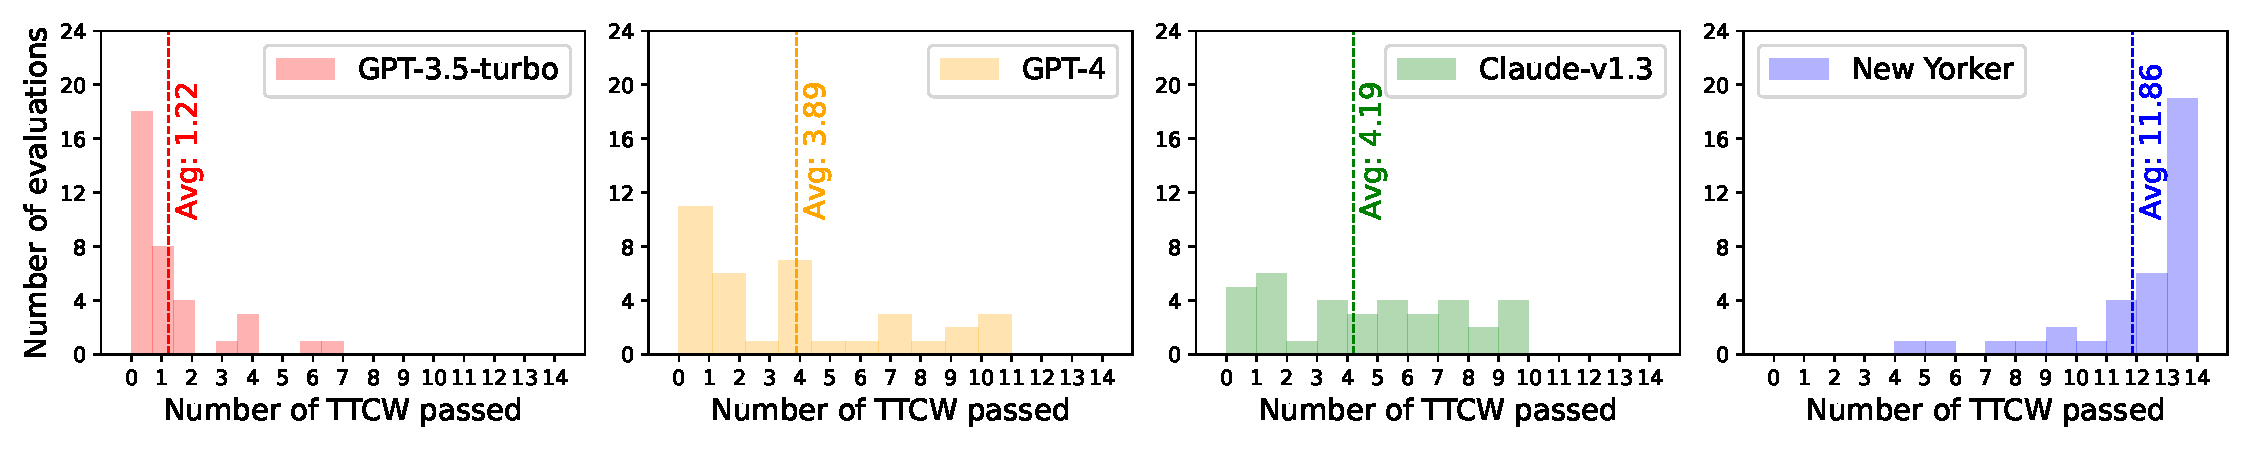
\includegraphics[width=0.95\textwidth]{figures/Creativity_Aggregate_Performance.pdf}
    \caption{Distribution of aggregate TTCW results, in which only the number of tests passed is retained. }
    \label{fig:ttcw_aggregate_histogram}
\end{figure*}

\begin{figure*}[!ht]
    \subfloat[Likert plot showing ranking of stories within an individual group based on all expert preferences]{\frame{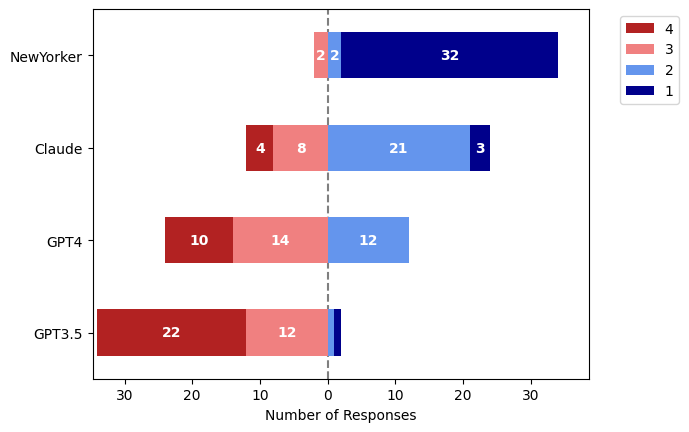
\includegraphics[width=0.44\textwidth]{figures/relativerank.png}}} \quad
    \subfloat[Likert plot showing how often authors attributed the source of the stories correctly]{\frame{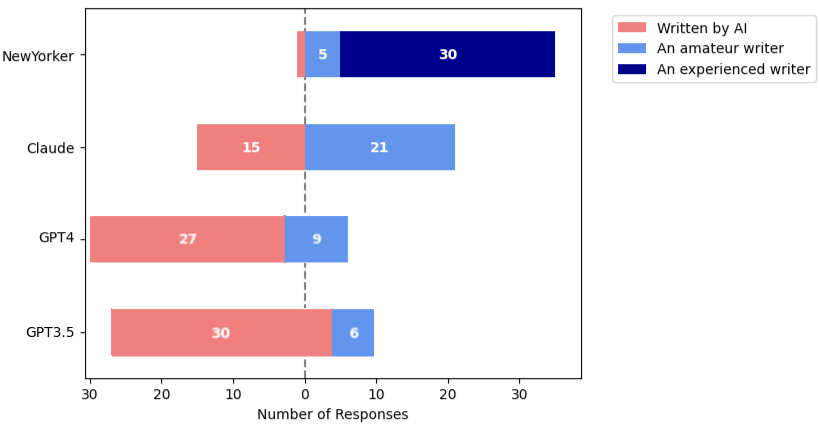
\includegraphics[width=0.53\textwidth]{figures/relativeauthor.png}}} 
    \caption{\label{relativehumaneval1} \textbf{Relative Evaluation} Left figure showing ranking preference assigned to each story within a group. Right figure showing how creative experts attributed any given story from The NewYorker or 3 LLMs to one of the options between An experienced writer, An amateur writer, or An AI }
\end{figure*}

Table ~\ref{absolutehumaneval} summarizes the average \textit{passing rate} on the 14 TTCW for each of the four story types (GPT3.5, GPT4, Claude-v1.3, and New Yorker). Passing rate here corresponds to the percentage of time expert participants answer `Yes' to an individual TTCW for any given story. The New Yorker stories widely achieve the highest passing rate on all fourteen tests, with an overall pass rate of 84.7\%. In other words, individual New Yorker stories are assessed to pass 11.9 of the 14 TTCW on average. When examining performance on individual tests, no test receives a pass rate of 100\%, confirming that no test is an absolute requirement in high-quality creative writing, and experimentally justifying the need to conduct the TTCW tests as a set (Design Principle 4).

Moving to the performance of the LLM-generated stories, passing rates are much lower, with GPT3.5 stories passing less than 10\% of TTCW, while GPT4 and Claude v1.3 are closer to 30.0\%. In other words, LLM-generated stories pass between a third and a tenth of the TTCW compared to human-written New Yorker stories. When breaking down LLM-story performance across the Torrance dimensions, all models achieve their highest pass rate on the Fluency dimension, and Claude v1.3 achieves the highest performance on average across Fluency, Flexibility, and Elaboration, while GPT4 scores highest on the Originality dimension. This experimental finding is surprising as Claude v1.3 is an LLM that is smaller in size(52B) than GPT4 \footnote{https://the-decoder.com/gpt-4-architecture-datasets-costs-and-more-leaked/}. 

\subsubsection{Reproducibility of TTCW}

Since we collected three independent TTCW evaluations for each story, we can report the agreement levels of experts when they conduct the tests individually, and their assessment in aggregate. We compute the Fleiss $\kappa$ agreement across all annotations and report the interrater agreement level of each test in Table ~\ref{absolutehumaneval}. Individual test agreement ranges from 0.27 to 0.66, and averages at 0.41, suggesting moderate agreement on most of the individual TTCW.

Since the TTCW are designed to be additive, we further compute an aggregate score for each story by counting the number of TTCW tests a story passes. We visualize the results of this aggregate measure in Figure ~\ref{fig:ttcw_aggregate_histogram}. Since the aggregate measure is numerical (ranges from 0 to 14), we use Pearson correlation to measure agreement among experts. At this aggregate level, we obtain a correlation($\rho$) of 0.69, showing strong agreement among experts on the number of tests a story passes. In other words, even though experts reach slightly lower agreement on which exact TTCW a story passes or fails, they achieve strong agreement on the number of tests a story passes overall. This experimental finding confirms the importance of Design Principle 4, and the need for the tests to be performed as a set to achieve a reproducible evaluation of creativity for a given short story. When the objective is to evaluate the broad creativity in a short story, we recommend that all fourteen tests be administered as a set by one expert annotator, rather than by different experts or administering only an individual test, as this increases the reproducibility of the results.
\subsubsection{Comparative Evaluation Results}

The final portion of the evaluation protocol asks expert participants to rank the four shuffled stories in terms of subjective preference, as well as guess each story's origin between ``An experienced writer'', ``An amateur writer'', or ``Written by AI''. Figure~\ref{relativehumaneval1} summarizes the results from this final portion of the study.

Looking at the ranking results, human-written New Yorker stories were ranked as the most preferred story 89\% of the time, while the GPT-3.5-generated stories ranked as least preferred roughly two-thirds of the time. When comparing GPT-4 and Claude, Claude is almost twice as likely to rank as second (behind the human-written story) and was the most preferred on three of the four assessments in which the New Yorker story was not chosen as the most favored. These ranking results confirm and accentuate the observation from the test passing rates analysis that Claude V1.3 generates higher-quality short stories than models in the GPT family.

The attribution results paint a similar picture, with New Yorker stories predominantly attributed to an experienced writer, while LLM-generated stories get attributed to AI or an amateur writer. Interestingly, Claude V1.3 is more likely to be attributed to an amateur writer than an AI, whereas GPT3.5 and GPT4 stories are 80\%+ attributed to AI. One hypothesis for such behavior could be that the participants in our study might be more familiar with text written by OpenAI models, as these models are commercially more successful, providing an element of surprise to Claude-generated text.

\subsection{What can we infer from expert explanations of administering the TTCW?} \label{sec:analysis}
\begin{table*}[ht]
\small
\centering
\def\arraystretch{1.2}
\begin{tabular}{|l|l|lll|}
\hline
\multirow{4}{*}{\begin{tabular}[c]{@{}l@{}}Originality\\ in Thought\end{tabular}} & NewYorker & \multicolumn{3}{l|}{\begin{tabular}[c]{@{}l@{}}The ideas in this piece are unique, and expressed with original language. The metaphorical \\ language referenced above is a list of good examples. Others include the moment when she\\ slides her sunglasses down and everything goes darker; Rabbi Adler's monotonous drone \\ rendered as--son...his...own...flesh; Barbara rocking like the overloaded boat she's become.\\ This piece is practically bursting with new, exciting ways of expressing familiar things.\end{tabular}} \\ \cline{2-5} 
 & Claude & \multicolumn{3}{l|}{While the piece avoids overused expressions, its ideas and themes are hackneyed.} \\ \cline{2-5} 
 & GPT4 & \multicolumn{3}{l|}{\begin{tabular}[c]{@{}l@{}}The characters in this piece are so defined by their religion and culture as to be flattened by \\ stereotype. The events of this piece feel arbitrary, almost random. While that does grant it an\\ unpredictability and a vague form of originality, it feels thoughtless.\end{tabular}} \\ \cline{2-5} 
 & GPT3.5 & \multicolumn{3}{l|}{\begin{tabular}[c]{@{}l@{}}The piece relies on cliched turns of phrase to express actions and thoughts. Reality hits \\ Barbara like a tidal wave; days turn to weeks (and weeks?) and months; she uses her \\ experience to "bridge divides" and "heal wounds".\end{tabular}} \\ \hline
\end{tabular} 
\vspace{2ex}
\caption{\label{expertfeedbackcluster}Expert explanations on stories from NewYorker, Claude, GPT3.5 and GPT4 for one of the Originality test.}
\vspace{-4ex}
\end{table*}
\begin{table*}[!ht]
\small
\centering
% \def\arraystretch{1.3}
\begin{tabular}{|l|l|l|}
\hline
Test & Passing Stories & Failing Stories \\ \hline
\begin{tabular}[c]{@{}l@{}}Understandability \\ \& Coherence\end{tabular} & \begin{tabular}[c]{@{}l@{}}Logical sequences, Interconnected details,\\ Rich character development, consistent\\ tone, Surprising yet earned conclusions, \\ Internal consistency in atmosphere and\\ symbolism\end{tabular} & \begin{tabular}[c]{@{}l@{}}Jumpy timelines, Unsatisfying endings, Undeveloped \\ plot points, Contradictory details, Illogical events, \\ Rambling prose, No overarching focus, Disjointed \\ Transition, Unclear Narration, Clichéd elements,\\ Inconsistent characterization\end{tabular} \\ \hline
\begin{tabular}[c]{@{}l@{}}Language \\ Proficiency \\ \& Literary \\Devices\end{tabular} & \begin{tabular}[c]{@{}l@{}}Utilize literary devices sparingly and directly,\\ enhancing the narratives that primarily draw \\ their strength from characterization and plot \\ rather than from highly figurative language.\end{tabular} & \begin{tabular}[c]{@{}l@{}}Attempts at figurative language come across as \\ overwrought, confusing, nonsensical. Subtlety and\\ restraint seem lacking, and the language choices \\ more often obscure rather than illuminate.\end{tabular} \\ \hline
\begin{tabular}[c]{@{}l@{}}Narrative\\ Pacing\end{tabular} & \begin{tabular}[c]{@{}l@{}}Adeptly manage time and pacing, varying \\ narrative rhythm, employing economic \\ language, skillfully transitioning between past\\ and present, creating suspense, mood, and interest\end{tabular} & \begin{tabular}[c]{@{}l@{}}Abrupt, jarring shifts in time or scene.Pacing that's\\ too slow/fast without purpose. Overly long descri-\\ ptions or passages. Events feeling randomly \\ ordered or disconnected\end{tabular} \\ \hline
\begin{tabular}[c]{@{}l@{}}Narrative\\ Ending\end{tabular} & \begin{tabular}[c]{@{}l@{}}Resolutions that weave earlier themes and\\ character perspectives into surprising yet \\ inevitable endings, leaving room for \\ interpretation\end{tabular} & \begin{tabular}[c]{@{}l@{}}Abrupt or unearned resolutions, overly moralistic \\ conclusions, unrealistic happy endings, unresolved \\ story threads, forced theme statements, narrative \\ disconnect, and unexpected surreal elements.\end{tabular} \\ \hline
\begin{tabular}[c]{@{}l@{}}Scene vs\\ Exposition\end{tabular} & \begin{tabular}[c]{@{}l@{}}Strategic balance of vivid scenes and concise \\ summaries, complementing each other to \\ enhance the narrative flow and reader experience\end{tabular} & \begin{tabular}[c]{@{}l@{}}Overreliance on summary leaves the narrative \\ ungrounded.Abrupt shifts between the two modes \\ prove confusing. Brief, underdeveloped scenes\\ fail to impact the reader.Overwrought scene \\ description obfuscates rather than illuminates\end{tabular} \\ \hline\hline
\begin{tabular}[c]{@{}l@{}}Emotional\\ Flexibility\end{tabular} & \begin{tabular}[c]{@{}l@{}}Harmonize interiority and exteriority, using \\ well-crafted transitions and narrative techniques\\ to convey character's inner states and external\\ actions, thereby fostering a deep connection\\ with the protagonist\end{tabular} & \begin{tabular}[c]{@{}l@{}}Unclear distinction between inner and outer realities, \\ Unrefined interior thoughts, insufficient external \\ grounding, cliched abstract language, an indistinct \\ mix of memory and metaphor with the present,\\ and underdeveloped character inner lives.\end{tabular} \\ \hline
\begin{tabular}[c]{@{}l@{}}Perspective\\ \& Voice\\ Flexibility\end{tabular} & \begin{tabular}[c]{@{}l@{}}Convincing \& diverse perspectives where \\ authors employ techniques such as nuanced \\ character development, authentic voice \\ crafting, detail-oriented storytelling, \&\\ efficient implication of perspectives, ensuring\\ a delicate balance between relatable \& \\ unlikeable traits\end{tabular} & \begin{tabular}[c]{@{}l@{}}Narrator's perspective dominates, and the other \\ characters are not portrayed convincingly as full human\\ beings with distinct viewpoints. While there are\\ some interesting moments, overall the story lacks truly\\ diverse perspectives that feel authentic and human.\end{tabular} \\ \hline
\begin{tabular}[c]{@{}l@{}}Structural\\ Flexibility\end{tabular} & \begin{tabular}[c]{@{}l@{}}Effective narrative turns that were surprising yet \\ believable, enhancing story depth, matching \\ themes and characters, increasing complexity\\ and stakes, aligning with the story’s style and \\ voice, and providing answers to previously raised\\ questions.\end{tabular} & \begin{tabular}[c]{@{}l@{}}Turns and surprises are ineffective, random, or\\ nonsensical rather than purposeful or appropriate.\\ While some stories sparked interest with an unusual\\ premise or relationship, they often failed to deliver \\ on the potential\end{tabular} \\ \hline
\end{tabular}
\vspace{2ex}
\caption{\label{expertexpl1}Common themes and issues found in expert explanations for tests focusing on TTCW-Fluency and TTCW-Flexibility}
\vspace{-5ex}
\end{table*}

Our annotation effort in Section~\ref{experteval} required experts to not only annotate for binary labels but also provide a justification paragraph accounting for their assessment. In Table~\ref{expertfeedbackcluster}, we provide examples of such justification for one of the TTCW tests for Originality. To gain insights into the main justifications experts provide for a story to pass or fail a TTCW test, we performed a manual thematic analysis of the expert justifications. We organized the results into a set of minimal phrases that often appear when a story passes or fails each TTCW test. Recent work has shown the utility of LLMs in clustering \cite{viswanathan2023large}. Based on these findings we asked the GPT4 model to cluster explanations across a given TTCW dimension into recurrent and broader representative themes. Three authors of the paper then manually verified these themes to ensure correctness. The outcome is summarized in Table~\ref{expertexpl1} for Fluency and Flexibility tests, and Table~\ref{expertexpl2} in the Appendix for Originality and Elaboration tests. The underlying themes found across the explanations reaffirm prior findings from \citet{ippolito2022creative} where writers found LLM-generated stories experiencing difficulty in maintaining a style/voice and easily reverting to tropes and repetition as well as those from \citet{mirowski2023cowriting} where screenwriters complained about the lack of subtext and character motivation.

\begin{table*}[!ht]
\small
\def\arraystretch{1.15}
\centering
\begin{tabular}{|l|l|}
\hline
E5 & \begin{tabular}[c]{@{}l@{}}\textbf{\color{blue}The AI rarely knew how to end a story} -- it would get bigger \& bigger in scope, leaving the characters behind \& talking\\ about their legacy and the community and the world at large. \textbf{\color{ForestGreen}Whenever the AI attempted metaphor or comparison, it}\\ \textbf{\color{ForestGreen}typically fell flat, with nonsensical analogies}. And it often didn't have a strong grasp on narrative structure; \textbf{\color{orange}characters} \\  \textbf{\color{orange}would sometimes appear without warning and then disappear without having any impact on the story itself}. The \\AI clearly knows the different elements of a story but doesn't have a grasp on how to merge them into a satisfying narrative.\end{tabular}                                                                                        \\ \hline
E3 & \begin{tabular}[c]{@{}l@{}}The story tends to use vague or cliched language, often repetitively. \textbf{\color{purple}Some words or phrases tended to be used again}\\ \textbf{\color{purple}and again over multiple stories for example ``\textit{inky sky},”  repeated a lot, as did ``\textit{etched}"}. There were parts that did not \\make sense over the course of the story. \textbf{\color{orange}A character might do something or think something in the beginning,}\\ \textbf{\color{orange}and then do something later that was contradictory or didn’t make sense}. Some of them were wildly trippy, like some\\ kind of surreal dream, in which nothing made sense.\textbf{\color{brown}The stories would spiral into a repetitive pattern, where the same}\\\textbf{\color{brown} things happened}, and the actions were described in similar ways. \textbf{\color{brown}It was as if the writer got stuck and just kept }\\ \textbf{\color{brown}repeating the same things}. This happened often when long periods of time passed.\end{tabular}                                                                                                                                                                      \\ \hline\hline
E4 & \begin{tabular}[c]{@{}l@{}}\textbf{\color{ForestGreen}Stories have over-modified descriptions but when AI does it, it's often followed by otherwise heightened diction} \\ in a way that human writing isn't. Sometimes, human writers will experiment with different syntax within their stories, but \\ I'd say, in my experience, it's somewhat rare. AI writing on the other hand demonstrated unusual/inconsistent syntax.Some\\ of the stories I believed were \textbf{\color{blue}AI-written had this weird forestalling of the ending}, which *could* happen with a novice \\ writer, for sure, but it didn't feel to me like a narrative choice a human writer would make. After the climax of the  story, \\\textbf{\color{blue}the falling action falls...and falls...and then just plateaus until the thing finally ends}\end{tabular}                                                                                                  \\ \hline\hline
E1 & \begin{tabular}[c]{@{}l@{}}\textbf{\color{ForestGreen}AI written sentences would be a series of words, positioned in a grammatically-correct fashion, with superficial}  \\ \textbf{\color{ForestGreen} shape that we associate with figurative language - but it just doesn't mean anything}. Figurative language adds \\meaning and context. It might be confusing, or poorly done, but there is always some idea being expressed in a non-literal\\ fashion. I've noticed that we, as real people, often answer questions in roundabout ways or ways that don't directly address \\the initial query. This brings a level of implied meaning or subtext to our conversations that hint at emotions and relationship\\ dynamics, something is often seen in high-quality fiction. However, \textbf{\color{red}I find AI-written dialogues disappointingly lacking}\\ \textbf{\color{red} in subtext}.They rely heavily on direct \& expositional dialogue, which feels decidedly unnatural \& less human. AI \textbf{\color{orange}characters}\\\textbf{\color{orange} frequently } \textbf{\color{orange} over-explain situations and emotions, resulting in an unrealistic portrayal of human interactions.}\\ Expert storytelling requires a nuanced understanding of reader engagement and artistic skill that amateur writers often \\lack, typically due to limited exposure to literature. This results in stories heavy in exposition and \textbf{\color{red}lacking in subtext}. AI\\-written stories take these issues to another level, often including random, incoherent elements and repeated pet phrases or\\ words.\textbf{\color{blue}These quirks become more} \textbf{\color{blue}noticeable over time, especially when AI attempts multiple disparate endings.}\\
Then consider the literal coherence of the stories. The definitely-AI ones would do random things \textbf{\color{orange}like introduce 'terrible }\\\textbf{\color{orange}beasts" who exist in the story for half a}\textbf{\color{orange} paragraph for some reason, and then just disappear.}
\textbf{\color{purple}There are also little}\\\textbf{\color{purple} pet phrases and words that repeat in the}\textbf{\color{purple}stories I am positive came from AI : a lot of "tendrils" and "inky}\\ \textbf{\color{purple}darkness."} And especially, a specific sentence construction of [time-orienting clause] [comma] [exposition].``\textit{In the days}\\\textit{that followed, X became a legend because Y.}" The same way authors have identifiable style and voice, so does AI.

\end{tabular} \\ \hline\hline
E2 & \begin{tabular}[c]{@{}l@{}}It seemed like there were two AI models that were generating stories for each batch. I feel like I began to notice and read\\ them as I would read or notice works by the same writer. \textbf{\color{brown} One would rapidly accelerate through time after the first}\\ \textbf{\color{brown} scene or so, probably once it was loose from the parameters it had been fed.}These accelerations were broadly pretty\\ absurd and hysterical. The other was a bit more subtle, but would \textbf{\color{blue}consistently end its stories  abruptly and employ}\\\textbf{\color{blue} somewhat bizarre logic}. In both cases, the \textbf{\color{red} AI seemed entirely unable to use implication or subtext}  \textbf{\color{ForestGreen}and its use of,}\\ \textbf{\color{ForestGreen} images, metaphors, etc was always very simple.}
\end{tabular}\\\hline
\end{tabular}
\vspace{2ex}
\caption{\label{expertfeedback}How do experts differentiate between AI vs. human-written stories?}
\end{table*}


\subsection{How do experts differentiate between human-written and LLM-generated stories?}
\label{expertvsai}

In an optional exchange with the expert participants (Section ~\ref{participant}) who participated in the annotation (Section ~\ref{experteval}), they were given the opportunity to describe how they differentiated between AI-generated and human-written stories. Collected responses showed that expert evaluators did not make a decision on which stories were AI-generated based on factors such as grammatical characteristics. Table \ref{expertfeedback} lists the replies of a few experts, which we color-coded to highlight the recurrent issues that led them to believe that a story is AI-generated. Feedback was often aligned with individual TTCW, demonstrating that experts discriminated AI vs human written stories based on creative execution rather than spurious cues.

In particular, E5, E4, E1 thought AI struggles at \textbf{\color{blue}\underline{Narrative Ending}}. E5 and E4 highlighted that AI-generated stories would forestall the ending by getting bigger in scope. E1 highlighted that AI-generated stories would have multiple disparate endings. E5, E4, E1, and E2 all highlighted that AI-generated stories would often contain abstruse and incoherent metaphors that do not add meaning or extremely cliched or simple metaphors thereby demonstrating poor \textbf{\color{ForestGreen}\underline{Language Proficiency and use of Literary Devices}}. E1 highlighted one such example in a story - \textit{However, she managed to laugh louder and louder until her laughter transformed into an embrace of the sun's atmosphere}.

E1 and E2 further highlighted that characters in AI-generated stories have poor \textbf{\color{red}\underline{Rhetorical Complexity}} and are often lacking in subtext. E1 further added that AI-generated stories operate in a nearly opposite and Drax-like fashion in which there is only literal meaning, and that literal meaning is often nonsensical, or at least presented without any of the context that might make it seem like something a human would say or do.
E1 highlighted an exchange below from an AI-generated story:

\begin{center}
    Sarah: \textit{``We've been avoiding the inevitable, Max. During our time here we've grown closer, and now that it's almost over, we can't just pretend like it never happened.''} \\
    Max:  \textit{``I understand, Sarah. But how do we move forward? How do we navigate this complexity without unraveling everything we've built?''}
\end{center}

where he exclaimed that these statements make hackish sense as clumsy exposition directed at the reader, and no sense at all as sentences spoken from one alleged human being to another.
Both E5, E3, and E1 agreed on poor \textbf{\color{orange}\underline{Character Development}} in AI-generated stories where a character would appear and then disappear without having any impact. E3 and E2 also highlighted issues in \textbf{\color{brown}\underline{Narrative Pacing}} where stories would either spiral into a repetitive pattern or rapidly accelerate through time after the first scene. E1 and E4 also highlighted \textbf{\color{purple}\underline{Unusual Syntax}} in sentence structure in AI-generated stories and repetition of certain words and phrases across stories.
